\documentclass[12pt]{article}
\usepackage{url}
\usepackage{setspace}               
\usepackage[superscript]{cite}      
\usepackage{graphicx}               
\usepackage[normalem]{ulem}   		
\graphicspath{ {Figures/} }         
\usepackage{caption} 
\usepackage{cite}
\usepackage{indentfirst} 
\usepackage{float}
\usepackage{subcaption}
\usepackage{amsmath}  	
\usepackage{amssymb}
\usepackage{bm}
\textwidth=6.5in                    
\oddsidemargin=0.0in                
\usepackage{listings}
\usepackage{listings}
\usepackage{fancyhdr}
\usepackage{longtable}
\usepackage{tcolorbox}
\usepackage{adjustbox}
\usepackage{lipsum}
\usepackage{float}
\usepackage{placeins}
\usepackage{booktabs}

\usepackage[table]{xcolor}
\pagestyle{fancy}
\fancyhf{}
\lhead{8-Ball Pool}
\rhead{Page \thepage}
\setlength{\skip\footins}{4cm}

\usepackage{color}   
\usepackage{hyperref}
\hypersetup{
    colorlinks=true,
    citecolor=black,
    linktoc=all, 
    linkcolor=black,
}

\begin{document}

\begin{titlepage}

\newcommand{\HRule}{\rule{\linewidth}{0.5mm}} 

\center 

\textsc{\LARGE North Creek High School}\\[1.0cm] 
\textsc{\Large Advanced Programming Topics Final Project Design Document }\\[1.0cm] 

\HRule \\[0.4cm]
{ \huge \bfseries 8-Ball Pool}\\[0.4cm] 
\HRule \\[1.5cm]


\begin{minipage}{0.4\textwidth}
\begin{flushleft} \large
Mohamed Morsy\\ Gautham Manigantan \\ 
\end{flushleft}
\end{minipage}

\bigskip

\begin{table}[H]
\centering
\begin{tabular}{|p{2cm}|p{2cm}|p{9cm}|}
\hline
Date & Revision & Release Notes\\
\hline
 3/21/2025& Rev 01 & Initial Release\\
\hline
 3/24/2025& Rev 02&Sketches added\\\hline 
\end{tabular}
\end{table}

\end{titlepage}

\newpage
%-----------------------------------------------------------------------
\tableofcontents

\newpage
%----------------------------------------------------------------------

%-----------------------------------------------------------------------------

\section{Project Description}

Our project is an 8-ball pool game similar to the one on Game Pigeon. This game requires a lot of strategical thinking and calculations to win. This project is made purely using Java and uses Swing for the visuals. The user will be able to interact with the browser using mouse clicks and drags, which will result in the cue stick hitting the cue ball. Swing will be used to animate the movement of the balls and the intensity of the shot meter. For more detail on how the game of billiards works, see \textbf{Section~\ref{sec:info}}.


\section{What is Pool/Billiards?} \label{sec:info}
Billiards, or "pool", as many know it, is a cue sport where there is a table with six pockets. There are 15 balls numbered 1 through 15, and 1 cue ball that's completely white. The 8-ball, a completely black ball, is in the center of the rack, which is a triangle that holds the balls at the start. The yellow 1-ball is put in the front of the rack, a random solid in one corner, and a random stripe in the other. The rest of the object balls' (non-cue balls) order doesn't matter. The rack is lined up at one end of the table, where the 1 ball (the front of the rack) is lined up with the foot spot. The foot spot is the spot where the 3 lines shown in \textbf{Figure~\ref{fig:footspot}} intersect. The rack is lifted, and the first player then performs the break shot, which is where they hit the cue ball from behind the headstring, a line that's similar to the one going through the footspot, but on the other side. For the break shot to be legal, at least four balls must hit the sides of the table, or a ball must be pocketed. If the 8-ball is sunk on the break, the player can re-rack (restart) or is spotted, where the 8-ball is placed on the footspot. If the first player misses, the second player attempts the shot to sink a ball, and the first to legally pocket a ball chooses to be solids (1-7) or stripes (9-15). A player will continue to keep shooting as long as they legally pocket their assigned ball type, but if they miss or do a foul, the opponent gets a turn. Fouls that are common and will be detected by our game include the following:

\begin{itemize}
    \item Failing to hit a ball
    \item Hitting the cue ball off of the table \protect\footnote{ A "scratch" means the cue ball goes into a pocket or jumps off the table \label{note:scratch}}
    \item Pocketing the cue ball \protect\footnote{ This is an example of a "scratch"}
    \item Hitting the opponents' group of balls first
    \item The cue ball not hitting a table side or pocketing a ball after contact
\end{itemize}
\space

If a foul is detected, then the opponent receives "ball-in-hand", where they can place the cue ball anywhere on the table (outside of the table is prevented). In order to win the game, a player must sink all of their assigned balls and then legally pocket the 8-ball at the end to win. However, if a scratch\textsuperscript{\ref{note:scratch}} occurs, then the opponent would receive ball-in-hand or the opponent wins if the scratch occurs while shooting at the 8-ball.


\FloatBarrier
% Figure 1 diagram
\begin{figure}[htbp]
    \centering
    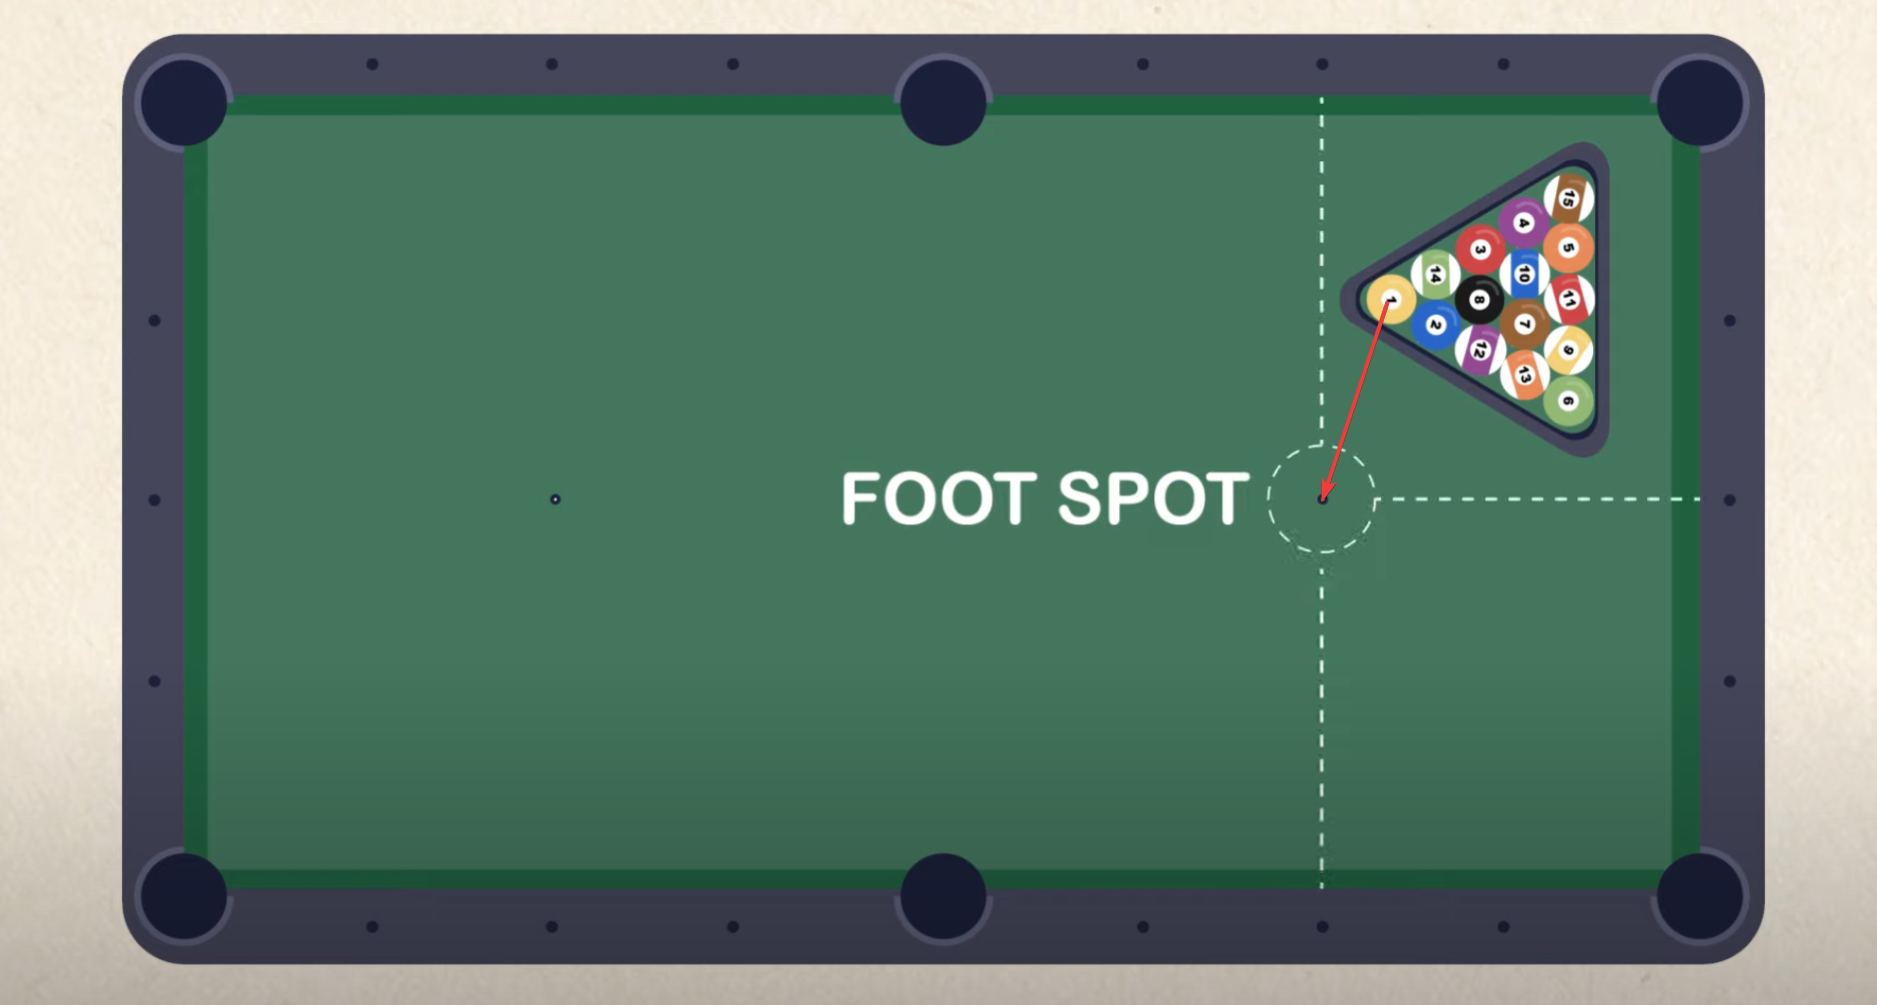
\includegraphics[width=0.7\textwidth]{footspot_diagram.png}
    \caption{The "foot spot" on a billiards table. Source: \href{https://www.youtube.com/watch?v=lmfKI01S-ws&ab_channel=wikiHow}{wikiHow on YouTube}.}
    \label{fig:footspot}
\end{figure}
\FloatBarrier

\section{Minimum Viable Product}

Our M.V.P. is a basic top-down two-dimensional game with a menu screen and game screen, where you can hold down and drag back a cue stick and let go to hit the ball in the direction the cue is facing.

\section{Purpose \& Motivation}

The purpose of the game is to help people enjoy time together playing a game they like. Many people can't afford to buy something like a pool table, and many online versions of pool aren't available to easily play with friends other than the one on Game Pigeon\protect\footnote{ Game Pigeon is an iOS mobile app that allows users to play mini games with each other through Message}. The problem with Game Pigeon is that it only works on iOS so this means that anyone who has an Android phone can't enjoy the game online with their friends. We want to solve this problem by making a 2 player 8-ball pool game that can be played anywhere offline with just 2 people. The motivation for this project was that we both really enjoy playing pool in person and online in Game Pigeon. We are also pretty interested in physics, so this allows us to combine our interests and put it into one game. Pool is also a very strategical game that is fun and simple at the same time so it is one of the most doable games in the short time frame.

\bigskip

\section{Core Features}

\begin{itemize}
    \item Interactive \& animated buttons that respond to clicks and make sound
    \item Accurate physical responses to ball collisions and hitting the ball with a cue
    \item User input handling (keyboard shortcuts and mouse clicks)
    \item Sound effects and music
    \item High quality graphics and user interface that is easily navigable and not distracting
    \item Dynamic and high quality animations for the objects in the game
\end{itemize}

\section{Additional or "Stretch" Features\protect\footnote{ Features are ranked by difficulty, top being the most difficult, and bottom being the least.}}

\begin{enumerate}
\item Custom algorithm-based AI mode that responds to user moves
    \item Different AI "bots" to play against that play with different difficulties?
    \item Game replays (moves are saved and replayed in game upon user response)
\item Tutorial mode that teaches the user how to play step-by-step (rather than an instructions page)
\item Statistics screen at the end with detailed information
\end{enumerate}

\section{Sweeping Algorithm}
If we have time, we plan to implement a sweeping algorithm for the game AI. The idea is that it's similar to a Bounding Volume Hierarchy, wherein the playing area is split into separate areas and each section is evaluated based on four categories of balls. A diagram is shown below, displaying the split up sections: A-F, and the four types of balls are in the top right corner. \textbf{S} is for striped, \textbf{N} is for non-striped, \textbf{C} is for cue ball, and \textbf{8} is for 8-ball. There are six circles indicating pocket locations on the rectangle that represents the billiard table. There are two line intersections that represent either footspot.

The steps for how the algorithm functions are as follows:

\begin{enumerate}
    \item Each separate area labeled A-F will be checked for the cue ball first. We set this found section as our Area of Interest (AoI). This will be checked by seeing if the coordinates of the cue ball are within the specified region. A visualization of this separation of regions can be shown in \textbf{Figure~\ref{fig:table}}.

    % Figure 3 diagram
    \begin{figure}[htbp]
        \centering
        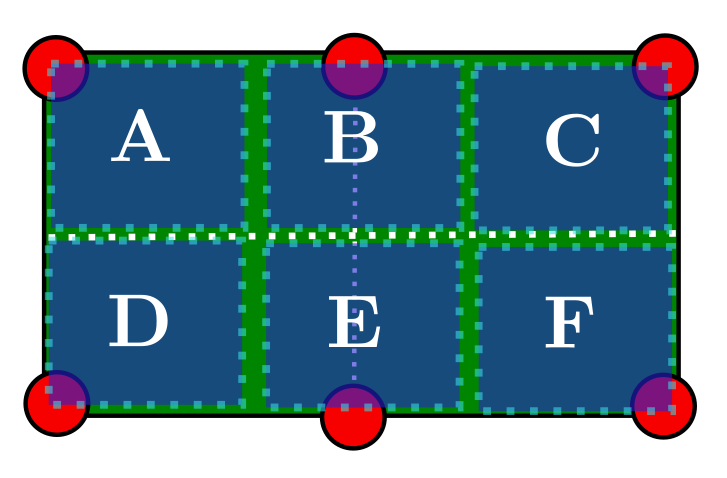
\includegraphics[width=0.85\textwidth ]{diagram_2.png}
        \caption{A visualization of the billiards table, with separate labeled regions A-F, and 6 pockets. }
        \label{fig:table}
    \end{figure}

    
    \item Then we "sweep" the area with a ray as shown in \textbf{Figure~\ref{fig:sweep}}, by about $\sim1^{\circ}$ at a time, checking to see if we've hit the cue ball\footnote{To address potential issues with whether or not the sweep will work, if the cue ball is at the center, then the sweep will circle around the ball, as when a path is first chosen, skipping the first step.}. The ray originates from the center of the AoI, and points outwards up until the edge of the square (unless it hits a ball). The magnitude of the ray increases slowly in order to account for a closer/farther cue ball


    \FloatBarrier
    % Figure 2 diagram
    \begin{figure}[htbp]
        \centering
        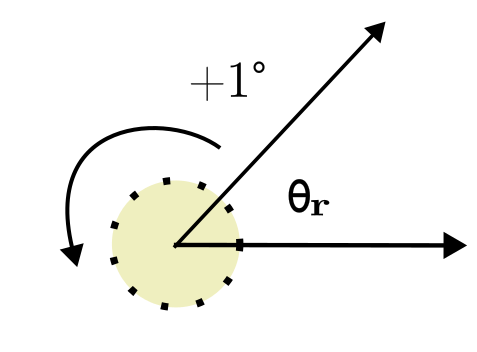
\includegraphics[width=0.7\textwidth]{diagram_1.png}
        \caption{The sweeping motion }
        \label{fig:sweep}
    \end{figure}
    \FloatBarrier
    
    \item Once that is complete, a second rotation is performed around the ball, beginning the process of choosing a path. To find a path, we continue in the same direction of the ray until we find a ball of the AI's type (let's say Stripes), and if not, until a pocket is found. If still not, alternate pathways are considered, which is explained further down the line. This process repeats with each subsequent ball, where the ray continues in the same direction as the reflection in a recursive process, where the exit condition is the force dampening factor has hit below 0.05 (our significance level). This is all for \textit{one} path, mind you.
    \item The reference angle from a line going right from the ball is saved for both the cue ball and next ball(s). The first angle is the shooting angle, denoted by $\theta_s$, and the rest are reference angles by a 0-th order, which we'll call $\theta_n$, where $n \in \mathbb{Z}, n\geq0$ and $n$ represents any positive integer value that is equal to or greater than 0. The reference angles will be saved in a Stack.
    \item Two other factors are considered: a force dampening factor, and alternate paths:
    \begin{itemize}
        \item The force dampening is a constant that represents how much more weakened the force will become as more collisions, friction, and distance traveled come into play (air resistance is negligible for our purposes). We define our net force equation on the ball using this dampening factor as shown:
        \begin{align}
        \Sigma F = \frac{(F_s - F_f)}{d_f} \\[1em]
        F_f = F_N \cdot C_{rr} \\
        F_N = m \cdot g \\[0.5em]
        D = \sqrt{(x_{b2}-x_{b1})^2 + (y_{b2}-y_{b1})^2} \\
        d_f = \frac{D}{(C_{rr} \cdot r_{b1})} \\
        \end{align}
        \item $\Sigma F$ represents the magnitude of the net force on the ball, $F_s$ is the "shooting" force applied by the user at some intensity, $F_f$ is the friction force, $C_{rr}$ is the coefficient of rolling friction of the billiard table, $F_N$ is the normal force, $d_f$ is the dampening factor, $m$ is the mass of the ball, $D$ represents the distance between the two balls using the distance formula, where $b2$ represents the second ball and $b1$ is the first, and $r_{b1}$ is the radius of the first ball. $F_D$ the drag force on the cue ball, where $C_d$ is the drag coefficient, which is about 0.47 for a sphere, $\rho$ is the air density at sea level, $A$ is the cross-sectional area of the ball, and $v$ is the velocity of the ball. (Note: $d_f$ must be between 0.0 and 1.0, and cannot be negative). To reference all of these values, here's a Reference Table:

        \begin{table}[h]
            \centering
            \begin{tabular}{ l c c }
                \toprule
                \textbf{Quantity} & \textbf{Symbol} & \textbf{Value (Units)} \\
                \midrule
                Gravitational Acceleration & $g$ & 9.81 m/s$^2$ \\
                Rolling Friction Coefficient & $C_{rr}$ & 0.01 - 0.03 (dimensionless) \\
                Radius of Cue Ball & $r_{b1}$ & 0.05715 m \\
                Mass of Cue Ball & $m$ & 0.17 kg \\
                \bottomrule
            \end{tabular}
            \caption{Reference Table of Physical Values Used in Equations Above}
            \label{tab:cueball_values}
        \end{table}
        
        \item A key point to mention is this is just the magnitude, and doesn't consider direction. Direction is determined using the Law of Reflection, wherein:
        \begin{align}
        \theta_i = \theta_r
        \end{align}

        \item $\theta_i$ represents the incident angle, or angle shot towards the ball, and $\theta_r$ is the reflected angle. They are congruent if measured from the normal, so therefore, for our purposes:
        \begin{align}
        \theta_r = 360^{\circ} - \theta_i
        \end{align}
        Where $\theta_i$ is measured as a reference angle just like $\theta_r$.

        \item As for the alternate pathways, lets say we recursed and could not find a ball to bounce off of or a pocket. Alternatives are then considered, such as hitting off of the wall and reflecting back, and then shooting a ray until we hit a ball of our type or a pocket. Maybe double reflections are considered. If there are no possible moves, the AI will "break the rules" and skip its turn.
    \end{itemize}
    
    \item A check is then performed, where now that the move is a possibility, we count the amount of pockets that will result from this. This will require, when evaluating a collision, checking if the collided ball will follow a pathway that leads to a pocket. The goal is to find a move with maximum pockets. If all balls have been pocketed, then the first step is changed, where now the AI is trying to find a section with the 8-ball and cue-ball, and attempts to make a final pocket (this is an exception to the typical algorithm).
    
    \item Finally, we repeat step 3, where we rotate once again around the ball, avoiding any other paths that have been evaluated, and count pockets for each. Each possible pathway is considered a branch in an unbalanced tree (See \textbf{Figure~\ref{fig:tree}}). The optimal path is chosen by the branch with the most pockets (saved as the value in each node). The leaf nodes represent the final move in the total moveset, and if one were to traverse the tree, it would essentially be a replay of all the AI's move (may be used as a replay feature).

    \FloatBarrier
    % Figure 4 diagram
    \begin{figure}[htbp]
        \centering
        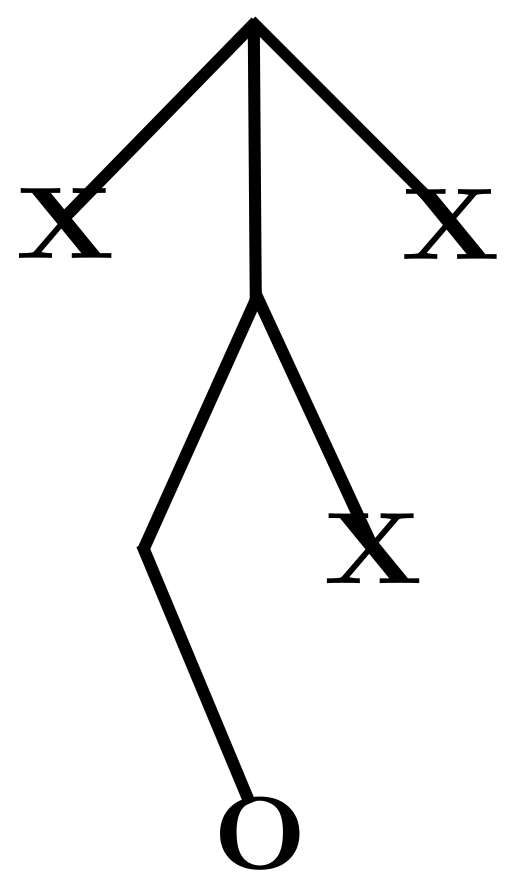
\includegraphics[width=0.7\textwidth]{diagram_3.png}
        \caption{An unbalanced tree that is scaled down to represent the various pathways the AI could take. The X's are cut off points, and the O represents the final leaf node where we have chosen a path. }
        \label{fig:tree}
    \end{figure}
    \FloatBarrier
    
\end{enumerate}

\section{Storyboard Sketches}
Here is a basic game screen flowchart indicating a rough idea of how the GUI (Graphical User Interface) for our game will look like:

\FloatBarrier
% Flowchart diagram
\begin{figure}[htbp]
    \centering
    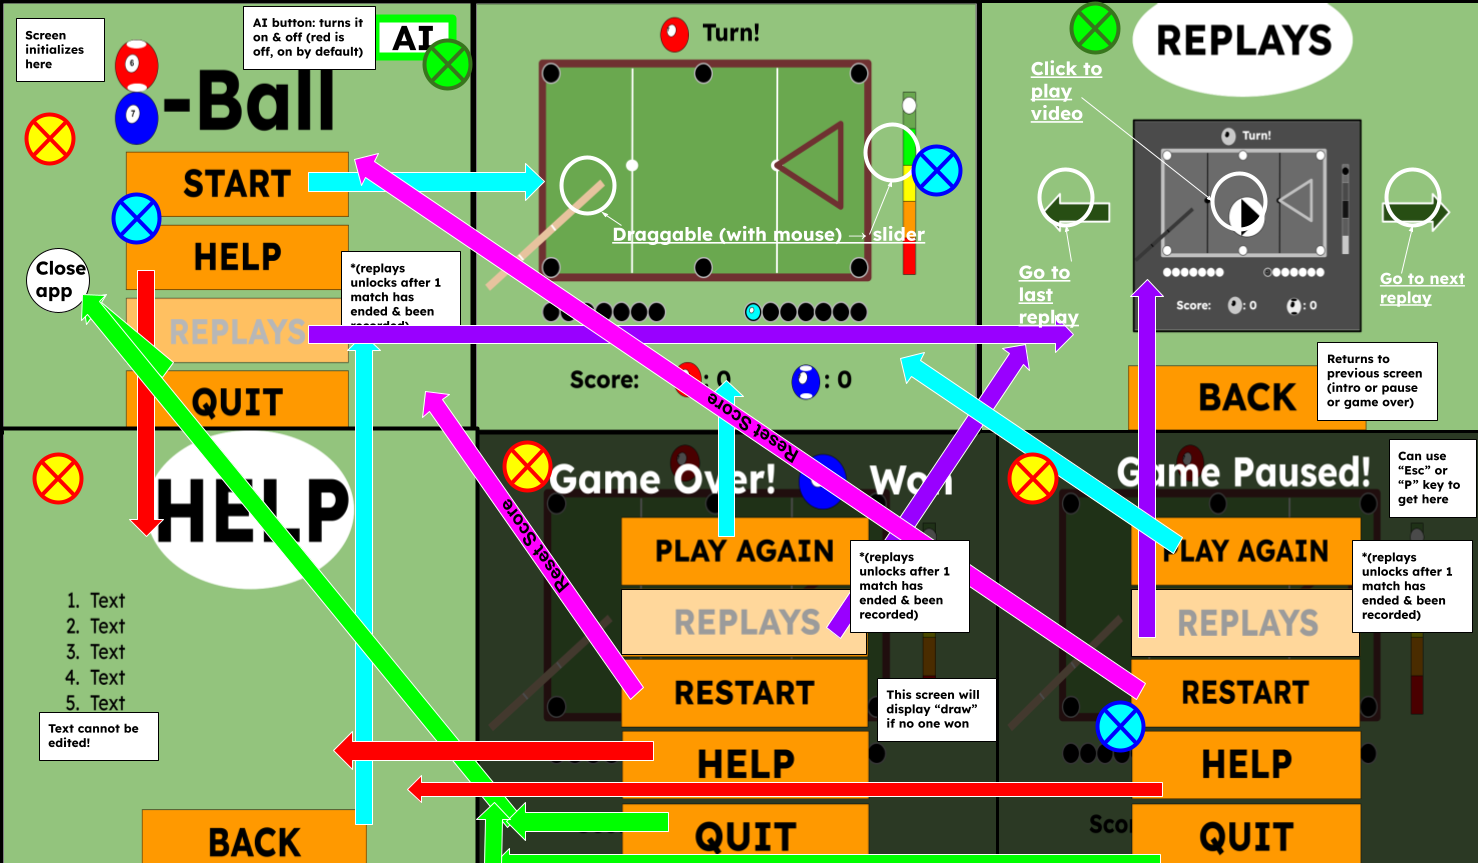
\includegraphics[width=0.7\textwidth]{diagram_flowchart.png}
    \label{fig:flowchart}
\end{figure}
\FloatBarrier

And here is a diagram of how the player will actually be able to interact with the game (mouse clicks, dragging, etc). \textbf{Note that all keystrokes from the player will be ignored (this is by design).}

\FloatBarrier
% Game Frames diagram
\begin{figure}[htbp]
    \centering
    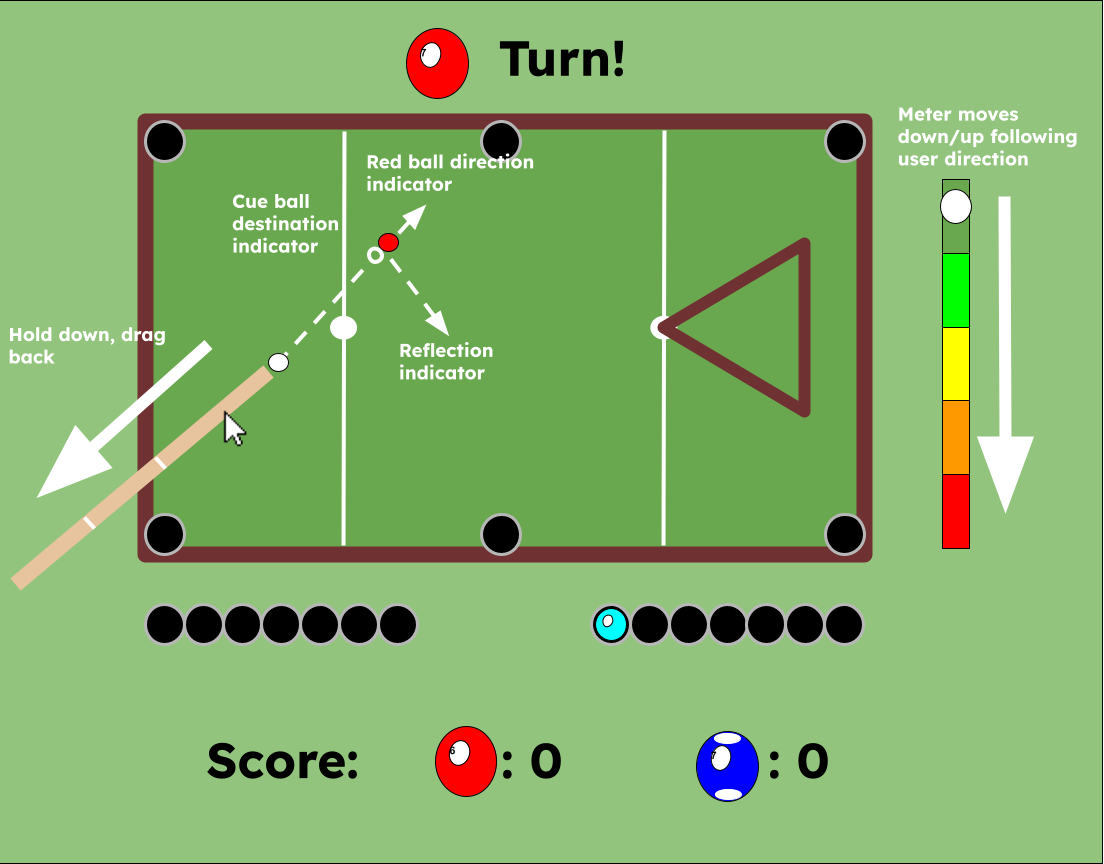
\includegraphics[width=0.7\textwidth]{diagram_gameframes.png}
    \label{fig:gameframes}
\end{figure}
\FloatBarrier


\newpage

\section{Learning Targets \& Challenge Goals}
Data Structures that will be used are a Stack for the reference angles, a Tree for the AI pathway algorithm, an ArrayList to save all balls on the screen currently, all balls for both the AI and Human that are pocketed or not, etc. We intend to use Java SwingUI, the Java Sound API, Canva, Visual Studio Code, Overleaf, JummBox, GitHub, and other technologies to design and create our project.
We hope to successfully implement a working menu screen, options/settings, AI debugging \& ray-tracing tools, as well as using the Java Preferences API to save user and game data, and Xuggle/Xuggler for audio and video recording for replays, and JavaFX Media with the Robot API to screenshot in the game.

\newpage
\clearpage

\end{document}


% May need to add conservation of momentum approach on top of the angle reflection?